% Chapter 4

\chapter{EXPERIMENTAL RESULTS AND PERFORMANCE ANALYSIS}
\label{ch:results}

This chapter describes the data and the computing environment used, the experiments conducted in Phase I, and an analysis of their results.

\section{DATASET DESCRIPTION}

\begin{table}[h!]
\centering
\caption{Dataset Description}
\label{tab:dataset}
\small
\renewcommand{\arraystretch}{1.3}
\begin{tabularx}{\textwidth}{|p{3.6cm}|L|}
\hline
\textbf{Attribute} & \textbf{Description} \\ \hline
Dataset & Visual Commonsense Reasoning (VCR)~\cite{zellers2019vcr}, Hugging Face release (Parquet files) \\ \hline
Source images & About 110,000 movie scenes from LSMDC~\cite{rohrbach2017lsmdc} and MovieClips \\ \hline
Questions & About 290,000 multiple-choice questions \\ \hline
Options & 4 candidate answers; 4 candidate rationales for the correct answer \\ \hline
Tasks & \QtoA, \QAtoR{} and the joint metric \QtoAR \\ \hline
Training set & VCR training split, 3 examples per question \\ \hline
Selection set & VCR validation questions, used only to choose the epoch \\ \hline
Test set & Separate held-out VCR validation questions \\ \hline
Knowledge source & ConceptNet 5.5~\cite{speer2017conceptnet}, local SQLite database \\ \hline
\end{tabularx}
\end{table}

\subsection{Visual Commonsense Reasoning (VCR) Dataset}
The VCR dataset~\cite{zellers2019vcr} contains about 290,000 multiple-choice questions over about 110,000 images taken from movie scenes, drawn from the LSMDC~\cite{rohrbach2017lsmdc} and MovieClips collections, as summarised in Table~\ref{tab:dataset}. Each question comes with four candidate answers and, for the correct answer, four candidate rationales. Objects and people in each image are detected and referred to in the text by tags, for example ``Why is [person1] pointing at [person2]?''. The questions cover explanations, activities, mental states, roles, temporal inferences and hypothetical situations, which makes them a close match to the activity, relationship and intention targets of this project. The wrong options are produced by Adversarial Matching, so they are relevant to the scene and cannot be rejected on surface cues alone.

\subsection{Data Splits Used}
Since the labels of the official VCR test split are not public, all evaluation questions are drawn from the official validation split. Three disjoint sets are used. The \textbf{training set} contains questions from the VCR training split, each expanded into a \QtoA, a \QAtoR{} and a free-form explanation example. The \textbf{selection set} of validation questions is used only to choose the epoch. The \textbf{test set} of further validation questions is used neither for training nor for choosing the epoch.

\subsection{ConceptNet Knowledge Base}
ConceptNet 5.5~\cite{speer2017conceptnet} is used as the commonsense knowledge source. A local SQLite database built from the ConceptNet assertions allows offline and reproducible lookups, with the public ConceptNet API and an on-disk cache as a fallback.

\subsection{Social Interaction Taxonomy}
The label space for the three prediction tasks is defined in \path{configs/taxonomy.yaml}. Each label has a description, a set of ConceptNet anchor concepts and a keyword lexicon. Examples of labels are \emph{Performing}, \emph{Watching together} and \emph{Photographing} for the activity; \emph{Performer or speaker and audience}, \emph{Teammates or members of the same group}, \emph{Doctor (or nurse) and patient} and \code{none\_single} for the relationship; and \emph{To entertain or perform for others}, \emph{To socialise, relax and spend time together} and \emph{To comfort, console or emotionally support someone} for the intention.
\subsection{Test Fixtures and Demonstration Data}
The automated tests use synthetic images, a deterministic stand-in for the VLM and a small ConceptNet graph, so they run without downloading the model. The qualitative demonstration uses real photographs, including the concert photograph of Section~\ref{sec:demo}.

\section{ECOSYSTEM}
\subsection{Hardware Configuration}
Fine-tuning was carried out on a GPU in the department laboratory, and the demonstration and interactive experiments were run on a local machine. The hardware configuration used is:
\begin{itemize}
    \item \textbf{Fine-tuning:} GPU workstation in the department laboratory (CUDA).
    \item \textbf{Inference and demonstration:} Apple Silicon MacBook, using the Metal Performance Shaders (MPS) backend of PyTorch.
    \item \textbf{Knowledge base storage:} local SQLite copy of ConceptNet on the inference machine, so no network access is needed at run time.
\end{itemize}

\subsection{Software Environment}
The system is organised as a Python package with separate modules for preprocessing, VLM inference, commonsense enrichment, reasoning, configuration, data structures and visualisation. The main software components used are:
\begin{itemize}
    \item \textbf{Programming Language:} Python 3.12
    \item \textbf{Image/Video Processing:} OpenCV~\cite{bradski2000opencv}, NumPy, PIL
    \item \textbf{Vision-Language Model:} SmolVLM with Hugging Face Transformers~\cite{wolf2020transformers}
    \item \textbf{Deep Learning Framework:} PyTorch~\cite{paszke2019pytorch}
    \item \textbf{Fine-Tuning:} PEFT (LoRA)
    \item \textbf{Natural-Language Processing:} spaCy and project text utilities
    \item \textbf{Commonsense Knowledge:} ConceptNet with SQLite database and cache
    \item \textbf{Backend:} FastAPI, Uvicorn
    \item \textbf{Frontend:} React, Vite, JavaScript
    \item \textbf{Testing:} pytest
    \item \textbf{Configuration:} YAML
\end{itemize}

\section{EXPERIMENTS CONDUCTED}

\subsection{Functional Validation Experiment}
The automated test suite was run with pytest to check each module and the complete pipeline. The preprocessing tests check image loading, resizing, normalisation, low-light enhancement, blur detection and frame sampling. The ConceptNet tests check term resolution, enrichment, label support and access to the local SQLite database, and further tests cover text normalisation and taxonomy loading. The end-to-end tests run the complete pipeline and check that commonsense evidence resolves the prediction when the VLM is uncertain, that scenes with one person or with no people are handled correctly, and that multiple-choice questions are answered. The video tests check key-moment selection and summarisation.

\subsection{LoRA Fine-Tuning Experiment}
SmolVLM was fine-tuned for 20 epochs with the configuration of Table~\ref{tab:ftconfig}, and the adapter was evaluated on the selection set after every epoch to choose the checkpoint.

\subsection{Quantitative Test Evaluation}
The base model and the selected fine-tuned model were evaluated on the same held-out test questions on \QtoA, \QAtoR{} and \QtoAR.

\subsection{Qualitative Comparison of Explanations}
The free-form answers and reasons of the base and fine-tuned models were compared for test questions against the reference answers.

\subsection{End-to-End Demonstration}
The integrated pipeline was run through the web interface on real photographs to inspect the predictions, the evidence and the processing time.

\section{PERFORMANCE ANALYSIS}

\subsection{Functional Validation Results}
All 23 automated tests passed, as summarised in Table~\ref{tab:tests}. These tests confirm that the module interfaces work together under controlled conditions: an input flows through preprocessing, VLM stand-in inference, ConceptNet enrichment and social reasoning to a structured prediction. Because the VLM is replaced by a deterministic stand-in, they validate the software, not the accuracy of the model; accuracy is analysed in the following sections.

\begin{table}[h!]
\centering
\caption{Automated Validation Results}
\label{tab:tests}
\small
\begin{tabular}{|l|c|c|}
\hline
\textbf{Test Category} & \textbf{Tests} & \textbf{Result}\\ \hline
Preprocessing & 7 & Passed\\ \hline
ConceptNet & 3 & Passed\\ \hline
Text and taxonomy & 5 & Passed\\ \hline
End-to-end Phase I pipeline & 5 & Passed\\ \hline
Video key-moment selection & 3 & Passed\\ \hline
\textbf{Total} & \textbf{23} & \textbf{23 Passed}\\ \hline
\end{tabular}
\end{table}

\subsection{Training Convergence}
The training loss is shown per optimiser step in Figure~\ref{fig:lossstep}, together with its moving average over 20 steps. Averaged per epoch, it falls from 2.03 in the first epoch to 0.08 in epoch 7 and 0.013 in epoch 11, and it is 0.001 or less from epoch 15 onwards. The loss therefore converges well before the end of the run.

\begin{figure}[H]
\centering
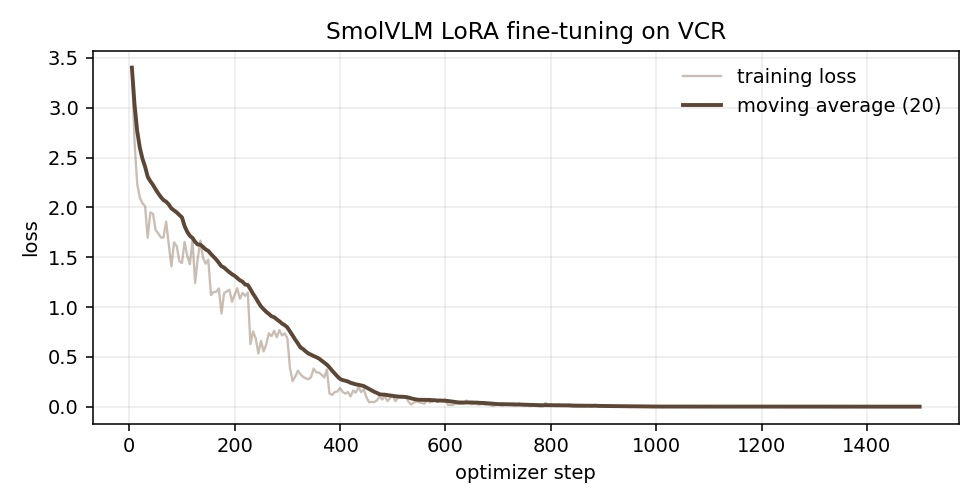
\includegraphics[width=\textwidth]{images/training_loss.png}
\caption{Training Loss of LoRA Fine-Tuning on VCR over 1,500 Optimiser Steps}
\label{fig:lossstep}
\end{figure}

\subsection{Epoch Selection}
The selection-set accuracy after every epoch is shown in Figure~\ref{fig:epochacc} and Table~\ref{tab:epochs}. Accuracy rises quickly over the first three epochs, with \QtoAR{} increasing from 33\% to 46\%, and then fluctuates between 43\% and 48\% while the training loss keeps falling. From epoch 12 onwards the accuracy is identical in every epoch, because the training loss is close to zero and the adapters no longer change.

Epochs 9 and 11 share the highest \QtoAR{} accuracy of 48\%. Epoch 11 is selected because its \QtoA{} accuracy is higher (63\% against 62\%), and its \QAtoR{} accuracy of 65\% is the second highest of the run. The final model therefore uses the epoch-11 adapter rather than the adapter from the last epoch.

\begin{figure}[H]
\centering
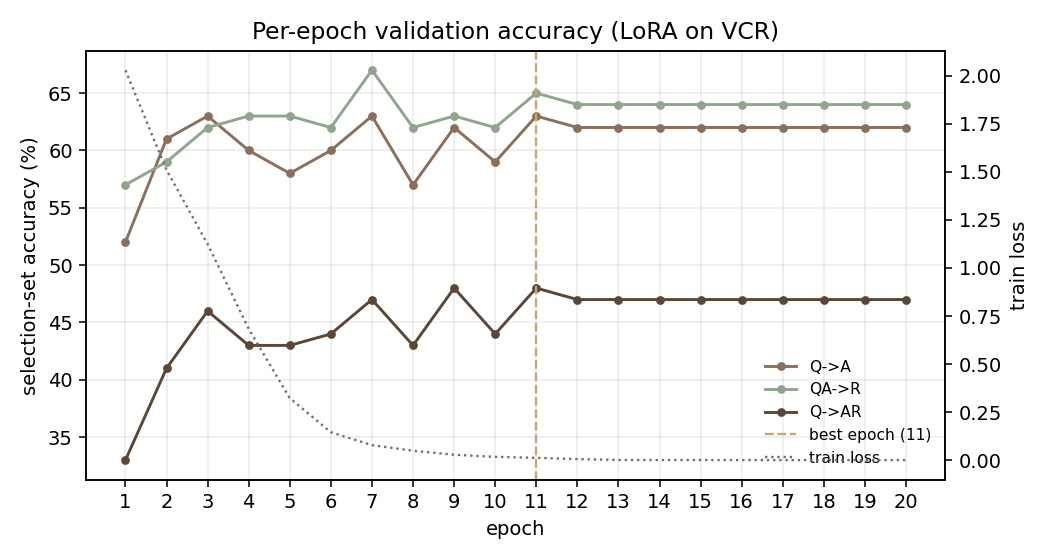
\includegraphics[width=\textwidth]{images/epoch_accuracy.jpg}
\caption{Selection-Set Accuracy and Training Loss after Each Epoch (Dashed Line: Selected Epoch 11)}
\label{fig:epochacc}
\end{figure}

\begin{table}[h!]
\centering
\caption{Per-Epoch Accuracy on the Selection Set}
\label{tab:epochs}
\small
\begin{tabular}{|c|c|c|c|c|}
\hline
\textbf{Epoch} & \textbf{Train Loss} & \textbf{\QtoA{} (\%)} & \textbf{\QAtoR{} (\%)} & \textbf{\QtoAR{} (\%)}\\ \hline
1 & 2.029 & 52 & 57 & 33\\ \hline
2 & 1.510 & 61 & 59 & 41\\ \hline
3 & 1.124 & 63 & 62 & 46\\ \hline
4 & 0.684 & 60 & 63 & 43\\ \hline
5 & 0.323 & 58 & 63 & 43\\ \hline
6 & 0.146 & 60 & 62 & 44\\ \hline
7 & 0.079 & 63 & 67 & 47\\ \hline
8 & 0.050 & 57 & 62 & 43\\ \hline
9 & 0.029 & 62 & 63 & 48\\ \hline
10 & 0.018 & 59 & 62 & 44\\ \hline
\textbf{11} & \textbf{0.013} & \textbf{63} & \textbf{65} & \textbf{48}\\ \hline
12--20 & 0.006 -- 0.001 & 62 & 64 & 47\\ \hline
\end{tabular}
\end{table}

The separation between the two curves -- training loss approaching zero while the selection accuracy stops improving after epoch 3 -- shows that the later epochs mostly fit the training examples more closely without generalising better. Selecting the epoch on held-out data, rather than using the last checkpoint, guards against this.

\subsection{Test Accuracy}
The base model and the fine-tuned model (epoch 11) were evaluated on the same held-out validation questions. Table~\ref{tab:testacc} and Figure~\ref{fig:testbar} give the results. Fine-tuning improves all three tasks by 14 to 17 percentage points, and the \QtoAR{} accuracy more than doubles, from 15.3\% to 32.7\%.

\begin{table}[h!]
\centering
\caption{Accuracy on Held-Out VCR Validation Questions}
\label{tab:testacc}
\small
\begin{tabular}{|l|c|c|c|}
\hline
\textbf{Model} & \textbf{\QtoA{} (\%)} & \textbf{\QAtoR{} (\%)} & \textbf{\QtoAR{} (\%)}\\ \hline
Chance level & 25.0 & 25.0 & 6.3\\ \hline
SmolVLM-Instruct (base) & 44.7 & 41.3 & 15.3\\ \hline
SmolVLM + LoRA (epoch 11) & \textbf{58.7} & \textbf{57.7} & \textbf{32.7}\\ \hline
Improvement (percentage points) & +14.0 & +16.3 & +17.3\\ \hline
\end{tabular}
\end{table}

\begin{figure}[H]
\centering
\begin{tikzpicture}
\begin{axis}[
  ybar, bar width=16pt, area legend,
  width=0.8\linewidth, height=6.5cm,
  symbolic x coords={qa,qar,qtoar},
  xtick=data, xticklabels={\QtoA, \QAtoR, \QtoAR},
  enlarge x limits=0.25,
  ymin=0, ymax=70, ylabel={Test accuracy (\%)},
  ymajorgrids, grid style={gray!20},
  axis line style={gray!60}, tick style={gray!60},
  every axis label/.style={font=\small}, ticklabel style={font=\footnotesize},
  nodes near coords, nodes near coords style={font=\footnotesize, color=black},
  every node near coord/.append style={/pgf/number format/fixed, /pgf/number format/precision=1},
  legend style={at={(0.5,1.03)}, anchor=south, legend columns=2, draw=none,
                font=\footnotesize, /tikz/every even column/.append style={column sep=10pt}},
]
\addplot[fill=neutralbar, draw=none] coordinates {(qa,44.7) (qar,41.3) (qtoar,15.3)};
\addlegendentry{SmolVLM-Instruct (base)}
\addplot[fill=seriesA, draw=none] coordinates {(qa,58.7) (qar,57.7) (qtoar,32.7)};
\addlegendentry{SmolVLM + LoRA (epoch 11)}
\end{axis}
\end{tikzpicture}
\caption{Test Accuracy of the Base and Fine-Tuned Models}
\label{fig:testbar}
\end{figure}

\subsubsection{Selection versus Test Accuracy}
The test accuracy is lower than the selection-set accuracy of epoch 11 (63\%, 65\% and 48\%). This is expected: the epoch was chosen because it scored well on the selection set, so its selection accuracy is optimistically biased. This is why the result is reported on a separate test set.

\subsubsection{Answer and Rationale}
If answer and rationale selection were independent, the expected \QtoAR{} accuracy would be the product of the \QtoA{} and \QAtoR{} accuracies: $0.587 \times 0.577 \approx 33.9\%$ for the fine-tuned model, close to the observed 32.7\%, and $0.447 \times 0.413 \approx 18.5\%$ for the base model, above the observed 15.3\%. Fine-tuning therefore improves both sub-tasks rather than only one, and the remaining errors are spread across both.

\subsubsection{Comparison with Published Results}
For reference, the R2C model reported 65.1\%, 67.3\% and 44.0\% (\QtoA, \QAtoR, \QtoAR) on the full VCR test set, and human performance was 91.0\%, 93.0\% and 85.0\%~\cite{zellers2019vcr}. These figures are not directly comparable with ours, which are on a held-out subset of the validation split, and R2C was trained on the full training set with detected object features. The comparison shows that a 2.2-billion-parameter general-purpose VLM, adapted with LoRA on a small amount of VCR data, reaches about three quarters of R2C's joint accuracy while also being able to generate free-form explanations, and that a large gap to human performance remains.

\subsection{Qualitative Comparison of Explanations}
Table~\ref{tab:qualitative} compares the free-form explanations of the two models for four test questions. For the violin and quarrel questions, the fine-tuned model gives the correct answer together with a visual reason, whereas the base model only describes what a person is looking at. For the father--son question, the base model states the relationship correctly while the fine-tuned model reverses it, although it gives the expected kind of reason (the age gap). For the dock question, neither model reaches the reference answer. The fine-tuned answers consistently follow the VCR pattern of an answer followed by its visual reason.

\begin{table}[h!]
\centering
\caption{Explanations of the Base and Fine-Tuned Models for Four Test Questions}
\label{tab:qualitative}
\small
\renewcommand{\arraystretch}{1.25}
\begin{tabularx}{\textwidth}{|p{2.3cm}|L|}
\hline
\multicolumn{2}{|l|}{\textbf{What is person2 doing?}}\\ \hline
Reference & He is playing a violin. He is holding a violin in one hand and applying the bow to it with the other.\\ \hline
Base & Looking at the ship.\\ \hline
Fine-tuned & He is playing a violin. He is holding a violin and a bow.\\ \hline
\multicolumn{2}{|l|}{\textbf{What is happening between person2 and person1?}}\\ \hline
Reference & They are quarreling. person2 looks tense and stern, person1 looks surprised.\\ \hline
Base & Person2 is looking at person1.\\ \hline
Fine-tuned & person1 is telling person2 something she doesn't like. person2 is looking at person1 with a stern expression.\\ \hline
\multicolumn{2}{|l|}{\textbf{How do person7 and person1 know each other?}}\\ \hline
Reference & person1 is person7's father. They came in together, and person1 is much older than person7.\\ \hline
Base & Person7 and person1 know each other. Person7 is the son of person1.\\ \hline
Fine-tuned & person7 is person1's father. There is a specific age gap between them, and they are going to embrace.\\ \hline
\multicolumn{2}{|l|}{\textbf{Why is person1 and person2 running on the dock?}}\\ \hline
Reference & They are trying to board a boat before it leaves. They won tickets on the boat they are trying to reach.\\ \hline
Base & Person1 and person2 are running on the dock because they are trying to catch person5.\\ \hline
Fine-tuned & person1 and person2 are trying to escape. person1 and person2 are running and person1 is carrying person2 up some stairs.\\ \hline
\end{tabularx}
\end{table}

The father--son example illustrates why Phase II is needed: an explanation can cite the right kind of evidence and still reach the wrong conclusion. Checking that the cited evidence corresponds to what the model attends to in the image, and that the textual and visual explanations agree, is the purpose of the cross-modal consistency and faithfulness evaluation.

\subsection{End-to-End Demonstration}
\label{sec:demo}
Figure~\ref{fig:uipred} shows the web interface analysing a photograph of a singer performing to a crowd at a concert. The system predicts the activity \emph{Performing} with 93\% confidence, the relationship \emph{Performer or speaker and audience} with 91\% and the intention \emph{To entertain or perform for others} with 97\% (Table~\ref{tab:demo}). In each case the next alternative receives 3\% or less, so none of the predictions is ambiguous. The generated explanation relates the prediction to visible evidence: the singer's outstretched arm and microphone, her smile, and the hands of the crowd reaching towards her.

\begin{figure}[H]
\centering
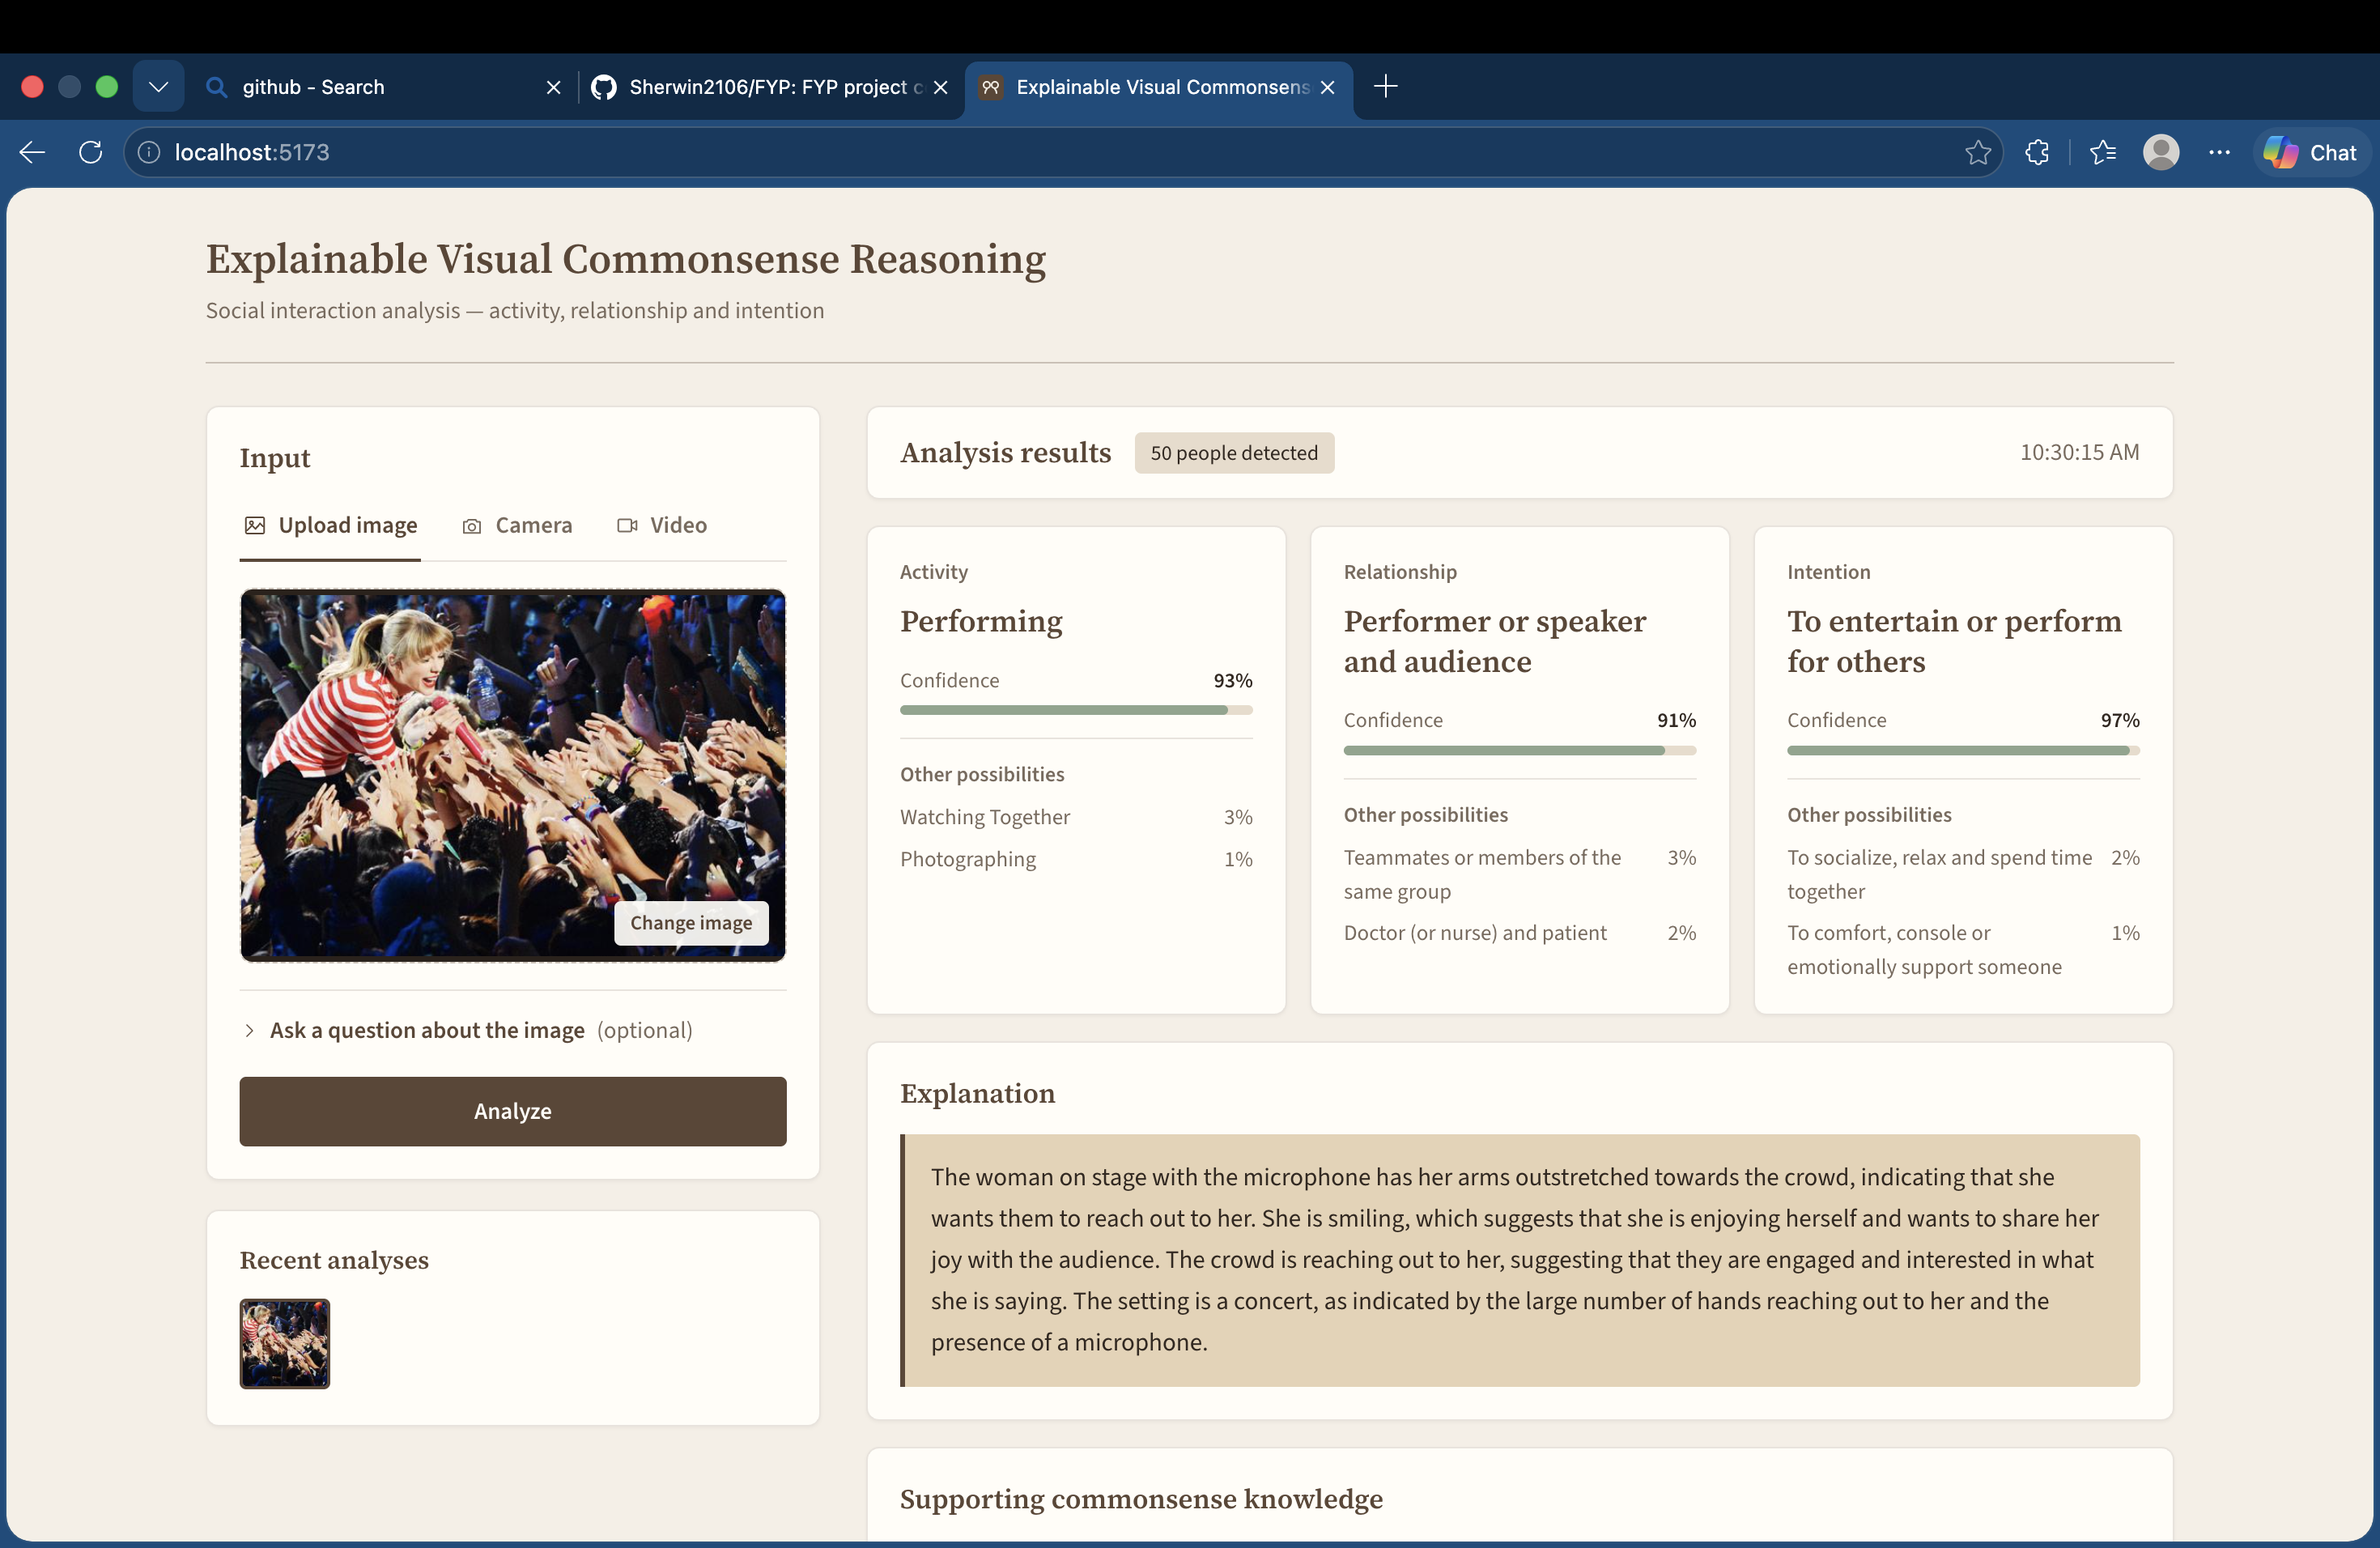
\includegraphics[width=\textwidth]{images/ui_predictions.png}
\caption{Web Interface: Predictions and Explanation for a Concert Photograph}
\label{fig:uipred}
\end{figure}

\begin{table}[h!]
\centering
\caption{Predictions for the Concert Photograph}
\label{tab:demo}
\small
\renewcommand{\arraystretch}{1.3}
\begin{tabularx}{\textwidth}{|p{2.6cm}|p{4.4cm}|c|L|}
\hline
\textbf{Task} & \textbf{Prediction} & \textbf{Conf.} & \textbf{Next Alternatives}\\ \hline
Activity & Performing & 93\% & Watching together (3\%), Photographing (1\%)\\ \hline
Relationship & Performer or speaker and audience & 91\% & Teammates (3\%), Doctor and patient (2\%)\\ \hline
Intention & To entertain or perform for others & 97\% & To socialise (2\%), To comfort someone (1\%)\\ \hline
\end{tabularx}
\end{table}

The supporting evidence and the scene description are shown in Figure~\ref{fig:uievid}. ConceptNet links the observed concepts to the predicted labels: ``concert'' and ``sing'' are closely associated with performing, a performer is typically found on a stage, and a concert is a kind of show. The VLM identified the setting as a concert, the actions as reaching out and holding up, the expressions as happy and excited, and the objects as a water bottle, a microphone and hands. The number of people reached the system's upper limit of 50, since the crowd is larger than that.

\begin{figure}[H]
\centering
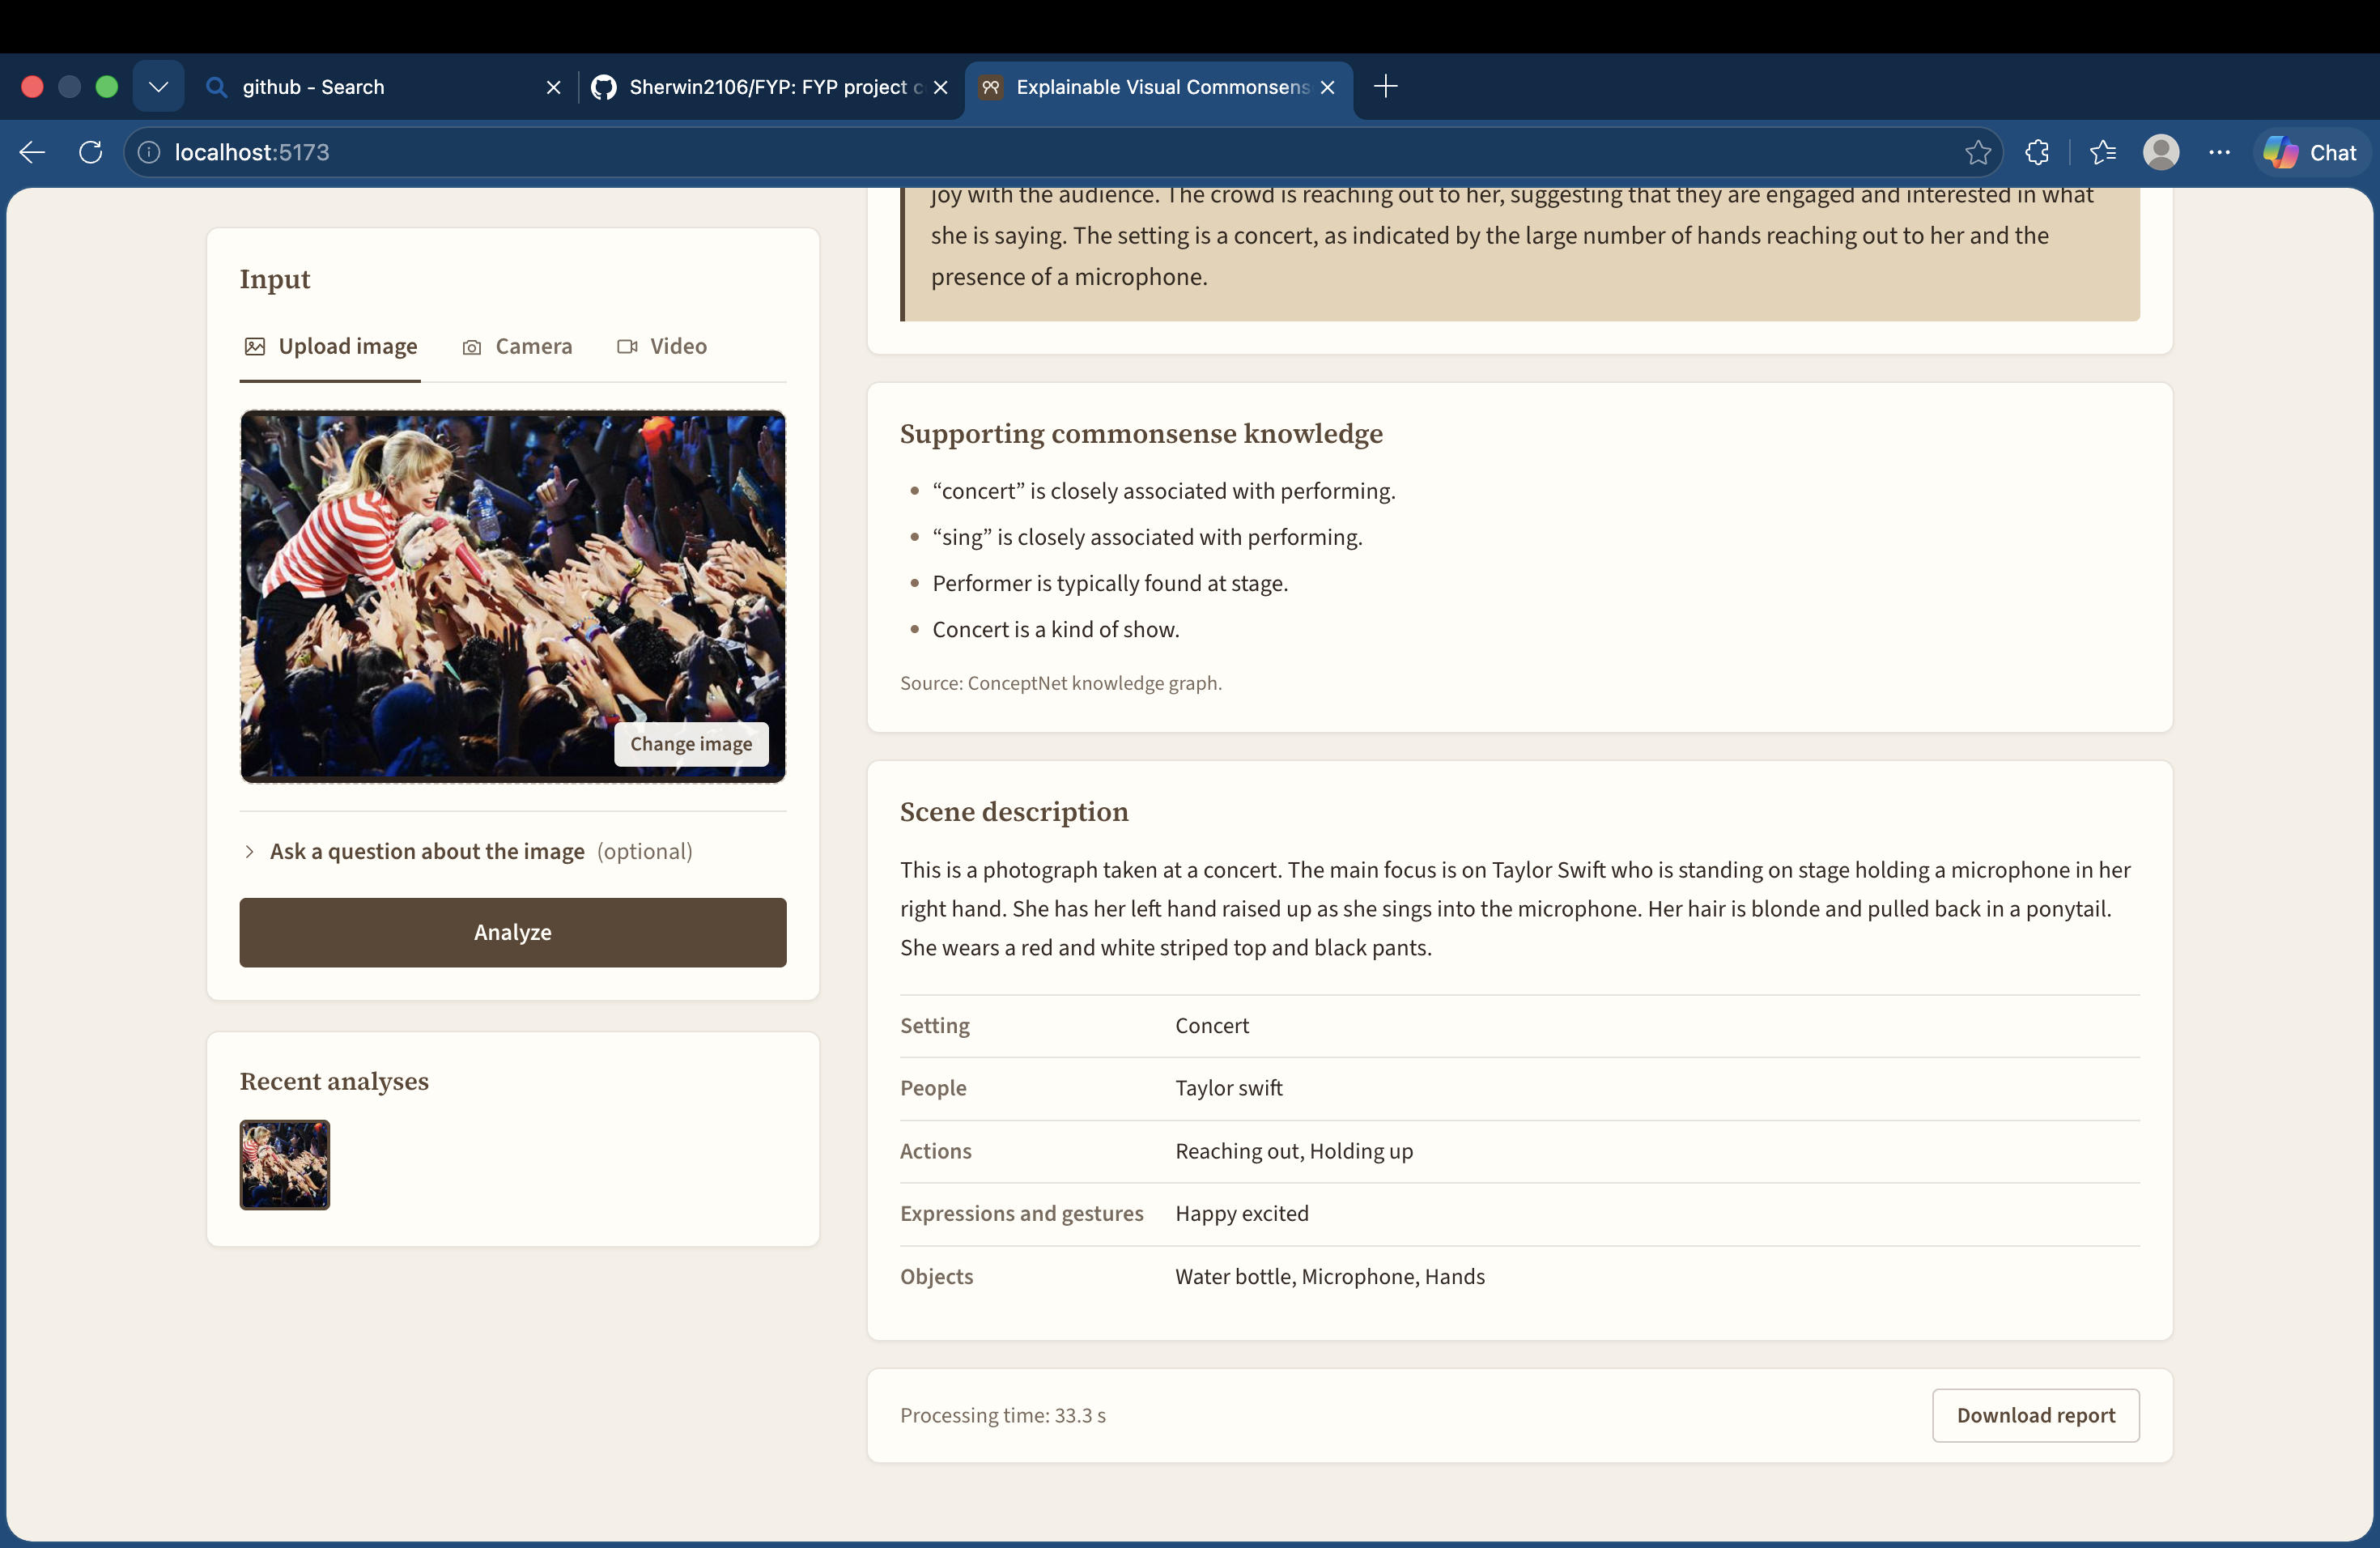
\includegraphics[width=\textwidth]{images/ui_evidence.jpg}
\caption{Web Interface: Supporting ConceptNet Knowledge and Scene Description}
\label{fig:uievid}
\end{figure}

The complete analysis of the concert photograph took 33.3 seconds on an Apple Silicon MacBook using the MPS backend. Most of this time is spent in the VLM: for a scene with two or more people and no question, Algorithm~\ref{alg:vlm} makes eleven generation calls, the explanation adds one more, and the option scoring of Algorithm~\ref{alg:mcscore} adds $k$ forward passes for each of the three tasks. The preprocessing and ConceptNet stages operate on small arrays and a local database, and contribute comparatively little. The per-module timings are recorded in every \code{Phase1Result}.

\subsection{Discussion}
Compared with a conventional image-captioning or classification pipeline, the Phase I system reasons at three levels. At the \emph{visual} level, it identifies the people, objects, actions, gestures and setting of the scene and describes them in a caption. At the \emph{commonsense} level, it links these observations to ConceptNet relations and label-support paths. At the \emph{decision} level, it fuses the VLM probabilities, the commonsense support and the draft match into a single prediction. The final prediction is therefore not a single sentence from the VLM: it retains the intermediate visual concepts, commonsense facts, component probabilities, alternatives and evidence that the explainability phase requires. Table~\ref{tab:status} summarises the status of each Phase I module.

\begin{table}[h!]
\centering
\caption{Phase I Implementation Status}
\label{tab:status}
\small
\renewcommand{\arraystretch}{1.3}
\begin{tabularx}{\textwidth}{|p{4cm}|p{2.2cm}|L|}
\hline
\textbf{Module} & \textbf{Status} & \textbf{Implemented Result}\\ \hline
Input and Preprocessing & Completed & Image/video/live input, quality checks, enhancement, resizing, normalisation and frame sampling\\ \hline
Small Vision-Language Model & Completed & SmolVLM integration, visual concept extraction, draft reasoning, deterministic generation and option scoring\\ \hline
Fine-tuning (offline) & Completed & LoRA fine-tuning on VCR for 20 epochs; epoch 11 selected; \QtoAR{} on held-out test questions raised from 15.3\% to 32.7\%\\ \hline
ConceptNet Commonsense Enrichment & Completed & Concept extraction, ConceptNet lookup, relevance filtering, label support, evidence and ambiguity resolution\\ \hline
Social Interaction Reasoning & Completed & Context fusion, activity/relationship/intention inference, log-linear fusion, confidence, alternatives and explanation generation\\ \hline
Explanation verification and dashboard & Phase II & Planned for the next phase\\ \hline
\end{tabularx}
\end{table}

\subsection{Limitations}
\begin{itemize}
\item The quantitative evaluation measures the fine-tuned VLM on VCR questions. There is not yet a labelled benchmark for the activity, relationship and intention predictions of the complete pipeline, so the end-to-end accuracy of the fused prediction has been assessed only qualitatively.
\item The fusion weights ($w_{\text{VLM}}$, $w_{\text{CN}}$, $w_{\text{draft}}$) and thresholds are set by hand; their effect has not yet been measured by an ablation study, and the calibration of the reported confidence values has not been measured.
\item The analysis of one image takes about half a minute, which is acceptable for single images but too slow for continuous real-time video.
\item The explanation is generated by the same VLM that makes the prediction, and its faithfulness has not yet been verified; this is the subject of Phase II.
\end{itemize}
